% 1998 上海理科第19题：直四棱柱及对角线/辅助线关系；示意图不按比例。
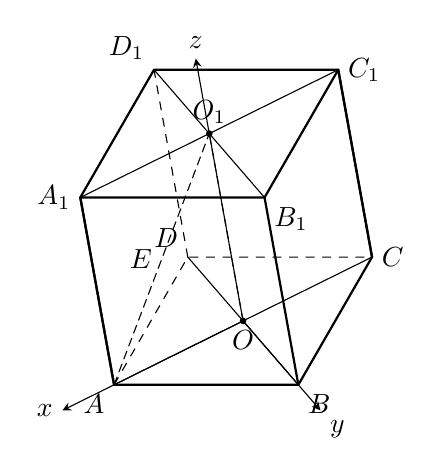
\begin{tikzpicture}[x=0.78cm,y=0.78cm,>=stealth,line cap=round,line join=round]
  \coordinate (A)  at (0,0);
  \coordinate (B)  at (3,0);
  \coordinate (C)  at (4.2,2.08);
  \coordinate (D)  at (1.2,2.08);
  \coordinate (A1) at (-0.55,3.05);
  \coordinate (B1) at (2.45,3.05);
  \coordinate (C1) at (3.65,5.13);
  \coordinate (D1) at (0.65,5.13);
  \coordinate (O)  at (2.1,1.04);
  \coordinate (O1) at (1.55,4.09);
  \coordinate (E)  at (0.775,2.045);
  % Prism edges; hidden base/side edges are dashed.
  \draw[thick] (A)--(B)--(C)--(C1)--(B1)--(A1)--cycle;
  \draw[thick] (A1)--(D1)--(C1);
  \draw[thick] (A)--(A1) (B)--(B1) (C)--(C1);
  \draw[dashed] (A)--(D)--(C) (D)--(D1);
  % Face diagonals intersect at O and O1; O1A passes through its midpoint E.
  \draw (A)--(C) (B)--(D) (A1)--(C1) (B1)--(D1);
  \draw[densely dashed] (A)--(E)--(O1) (O)--(O1);
  \fill (O) circle (1.2pt);
  \fill (O1) circle (1.2pt);
  \node[below left] at (A) {$A$};
  \node[below right] at (B) {$B$};
  \node[right] at (C) {$C$};
  \node[above left] at (D) {$D$};
  \node[left] at (A1) {$A_1$};
  \node[below right] at (B1) {$B_1$};
  \node[right] at (C1) {$C_1$};
  \node[above left] at (D1) {$D_1$};
  \node[below] at (O) {$O$};
  \node[above] at (O1) {$O_1$};
  \node[left] at (E) {$E$};
  % Coordinate rays point from O along OA, OB, and OO_1 as specified.
  \coordinate (xAxisEnd) at (-0.84,-0.416);
  \coordinate (yAxisEnd) at (3.36,-0.416);
  \coordinate (zAxisEnd) at (1.33,5.31);
  \draw[->] (O) -- (xAxisEnd) node[left] {$x$};
  \draw[->] (O) -- (yAxisEnd) node[below right] {$y$};
  \draw[->] (O) -- (zAxisEnd) node[above] {$z$};
\end{tikzpicture}
